\subsubsubsubsection{Urban Entity}
\begin{figure}[h]
\centering
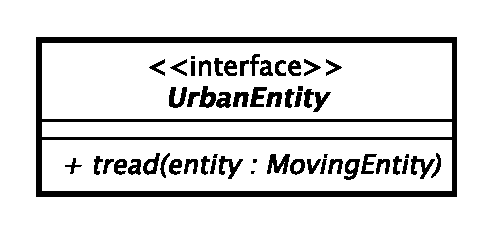
\includegraphics[scale=0.6,keepaspectratio]{images/solution/urban_entity.eps}
\caption{App::Reactive::Urban Entity}
\label{fig:sd-app-urban-entity}
\end{figure}
\FloatBarrier
\begin{itemize}
  \item \textbf{Description} \\
    It represents an entity that compose the district infrastructure.
  \item \textbf{Operation}
  \begin{itemize} 
    \item \texttt{\textit{+ tread(entity: MovingEntity)}} \\
Abstract method which will implement the treading of the moving entity 
on the urban infrastructure.
  \end{itemize}
\end{itemize}
